\pgfplotsset{width=8cm,compat=1.8}
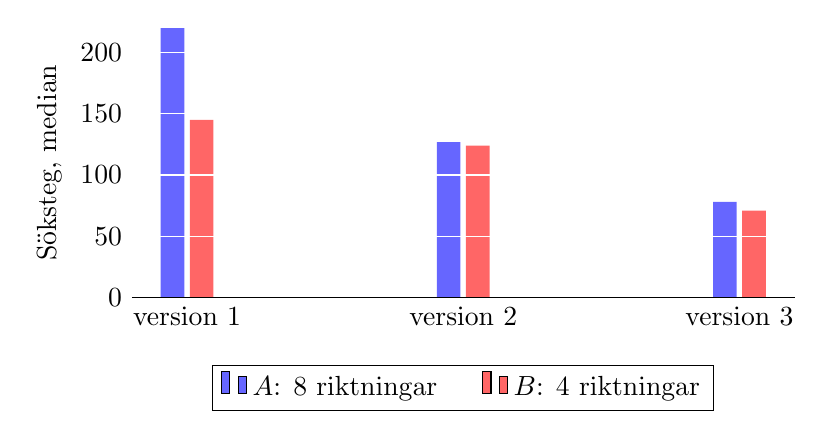
\begin{tikzpicture}
    \centering
    \begin{axis}[
        ybar,
        axis on top,
        % title={Söksteg algoritmer},
        height=5cm, width=10cm,
        bar width=0.3cm,
        ymajorgrids, tick align=inside,
        major grid style={draw=white},
        enlarge y limits={value=.1,upper},
        ymin=0, ymax=200,
        axis x line*=bottom,
        axis y line*=left,
        y axis line style={opacity=0},
        tickwidth=0pt,
        enlarge x limits=true,
        legend style={
            at={(0.5,-0.25)},
            % font=\footnotesize,
            anchor=north,
            legend columns=2,
            /tikz/every even column/.append style={column sep=0.5cm}
        },
        ylabel={Söksteg, median},
        symbolic x coords={version 1, version 2, version 3},
        xtick=data,
        % tick label style={font=\footnotesize},
        ]
        
        %% Median 8 riktningar
        \addplot [draw=none,fill=blue!60] coordinates {
            (version 1,224)
            (version 2,127) 
            (version 3,78)
        };

        %% Median 4 riktningar
        \addplot [draw=none, fill=red!60] coordinates {
            (version 1,145)
            (version 2,124) 
            (version 3,71)
        };
        \legend{$\mathscr{A}$: 8 riktningar,$\mathscr{B}$: 4 riktningar}
    \end{axis}
\end{tikzpicture}